\documentclass[12pt, a4paper]{article}

\title{Sistemi Operativi}
\date{}


\usepackage[margin=1in]{geometry}  % set the margins to 1in on all sides
\usepackage{graphicx}              % to include figures
\usepackage{amsmath}               % great math stuff
\usepackage{amsfonts}              % for blackboard bold, etc
\usepackage{amsthm}                % better theorem environments
\usepackage{wrapfig}			   % for images formatting
\usepackage{booktabs}
\usepackage{caption}			   % for labeling images
\usepackage{bigints}			   % for bigger integral symbols
\usepackage{listings}			   % coding environment
% \usepackage{minted}				   % code with colors
\usepackage{subcaption}			   % subfigures functions

% various theorems, numbered by section

\newtheorem{thm}{Theorem}[section]
\newtheorem{lem}[thm]{Lemma}
\newtheorem{prop}[thm]{Proposition}
\newtheorem{cor}[thm]{Corollary}
\newtheorem{conj}[thm]{Conjecture}

\DeclareMathOperator{\id}{id}

\newcommand{\bd}[1]{\mathbf{#1}}  % for bolding symbols
\newcommand{\RR}{\mathbb{R}}      % for Real numbers
\newcommand{\ZZ}{\mathbb{Z}}      % for Integers
\newcommand{\col}[1]{\left[\begin{matrix} #1 \end{matrix} \right]}
\newcommand{\comb}[2]{\binom{#1^2 + #2^2}{#1+#2}}

\begin{document}
	
	\section*{Lezione 3 (Processes)}
	
	Gestione dei processi:
	\begin{itemize}
		\item Inizialmente implementato totalmente \textit{batch}
		\item Successivamente viene implementata la multiprogrammazione ed il time-sharing e da quel punto nacque il concetto di \textit{processo}
		\item Un processo rappresenta un programma in esecuzione caratterizzato da sequenze di istruzioni, stato della CPU, variabili del programma e `return  addresses` correlati alle funzioni.
	\end{itemize}
	
	Per Von-Newmann ogni processo deve esistere nella memoria principale. 
	\begin{figure}[!htbp]
		\centering
		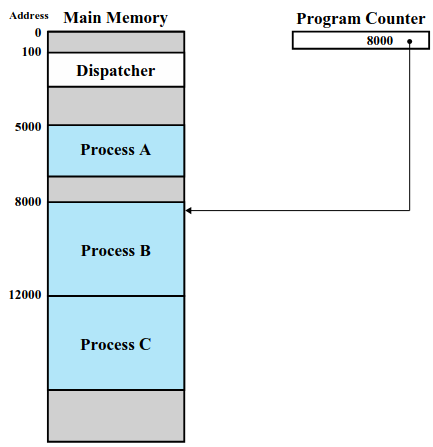
\includegraphics[width=8cm]{SO_PNGs/three-processes_SO.png}
		\caption*{}
		\label{fig:three-processes}
	\end{figure}
	
	
	Il SO legge gli eseguibili e ne costruisce le strutture dati in memoria principale \\
	Si usa un diagramma di stato per descrivere le fasi di esecuzione di un process:
	\begin{itemize}
		\item \textbf{New}: il processo viene creato e le strutture dati vengono inizializzate	
		
		\item \textbf{Running}: nei sistemi ``uniprocessore'', solo un processo per volta può essere eseguito
		
		\item \textbf{Ready}: il processo è \textbf{pronto} ma la CPU è momentaneamente in uso
		 
		\item \textbf{Blocked}: il processo è in attesa di un \textbf{evento}
		
		\item \textbf{Exit}: i risultati vengono rilasciati e le strutture dati vengono aggiornate
	\end{itemize}
	Il processo viene creato in Memoria Principale, se il processo viene effettivamente creato passa in stato di \textbf{Pronto}, ci sarà poi un ciclo di \textbf{Dispatch} o di \textbf{Timeout}(nel caso si dovesse eseguire un altro processo). Lo stato di \textbf{Bloccato} sta aspettando l'input di un certo evento e si sblocca una volta che l'evento avviene. Dopo l'evento lo stato torna in \textbf{pronto}.
	
	\begin{figure}[!htbp]
		\centering
		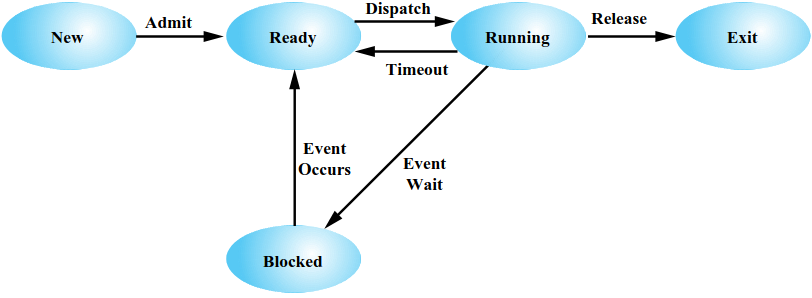
\includegraphics[width=14.5cm]{SO_PNGs/five-state-process-model_SO.png}
		\caption*{}
		\label{fig:five-state-model}
	\end{figure}

	\newpage
	
	
	\subsection*{Immagine del Processo} 
	Ogni sistema operativo ha il suo modo specifico di visualizzare le strutture dei processi. Per esempio in \textit{linux} viene visualizzato nel formato \textbf{ELF} (Executable and Linkable Format), \textbf{BF} nel caso di \textit{Windows}.
	
	
	\begin{figure}[!htbp]
		\centering
		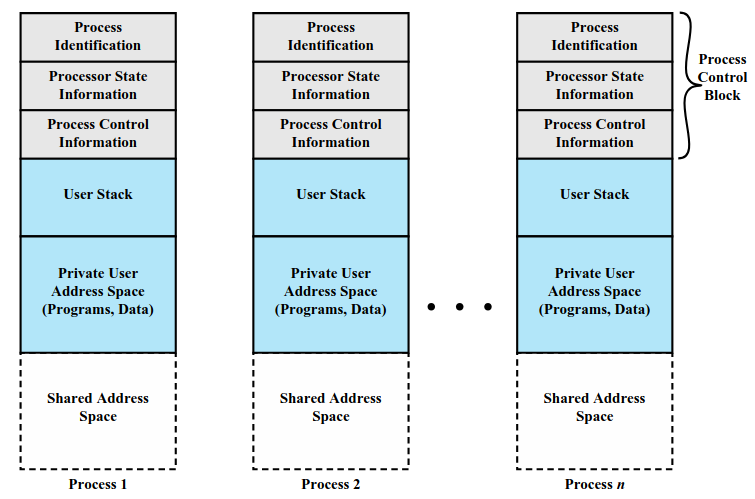
\includegraphics[width=15cm]{SO_PNGs/process-image_SO.png}
		\caption*{}
		\label{fig:process-image}
	\end{figure}
	
	\begin{wrapfigure}{r}{0.20\textwidth}
		\centering
		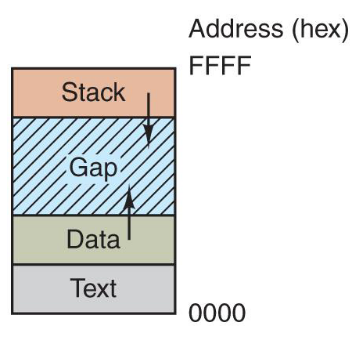
\includegraphics[width=3.8cm]{SO_PNGs/process-image-segments_SO.png}
		\caption*{}
		\label{fig:process-image-segments}
	\end{wrapfigure}
	
	Three main segments:
	\begin{itemize}
		\item the \textbf{text} segment the sequenze of the binary instructions of the program
		
		\item the \textbf{data} segment contains all initialized data
		
		\item the \textbf{gap} segment contains the \textbf{heap} where unitialized or dynamically allocated variables are stored
		
		\item the \textbf{stack} contains the \textbf{return addresses} for function calls
	\end{itemize}

	\begin{figure}[!htbp]
		\centering
		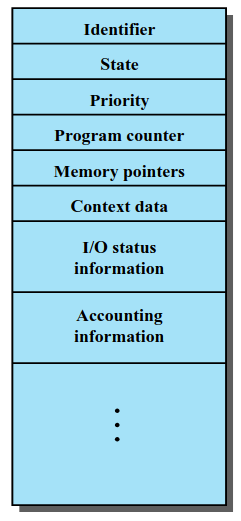
\includegraphics[width=4cm]{SO_PNGs/process-control-block_SO.png}
		%\caption*{}
		\label{fig:process-control-block}
	\end{figure}

	La PCB contiene le informazioni necessarie dal SO per identificare i processi e controllarne l'esecuzione \\\\
	
	\subsection*{Creazione dei processi} 
	Un processo viene creato da un'altro processo in esecuzione, il nuovo processo viene chiamato \textbf{processo figlio} ed il processo chiamante viene chiamato \textbf{processo genitore}. Ogni processo viene identificato da un numero (detto PID)\\
	Il processo genitore può condividere le risorse con il processo figlio mediante locazioni di memoria, files aperti, canali di comunicazione,... \\
	Dopo che il figlio viene creato, il processo genitore continua la sua esecuzione finché il SO non cambia al figlio, il genitore dovrà successivamente \textit{aspettare} fino alla completa esecuzione del processo figlio
	
	Tutti i programmi terminano con una chiamata ad \textit{exit}()
	
	
%	\section*{Lezione 4 (...)}
	
	
	\section*{Lezione 5}
	
	\subsection*{Process Scheduling} 
	\begin{itemize}
		\item \textbf{Multiprogramming}: Massimizza l'utilizzo della CPU
		\item \textbf{Time-sharing}: La CPU viene condivisa attraverso diversi processi ed utenti e l'obiettivo è minimizzare il tempo di risposta per ogni processo.
		\item \textbf{Scheduler}: è una delle componenti principali del SO. Ogni volta che un processore è in stato di \textit{idle}, lo scheduler seleziona uno dei processi in ready queue
		\item \textbf{Dispatcher}: Seleziona la task successiva, nel modo più veloce ed efficiente possibile, dalla ready queue
	\end{itemize}

	\begin{figure}[!htbp]
		\centering
		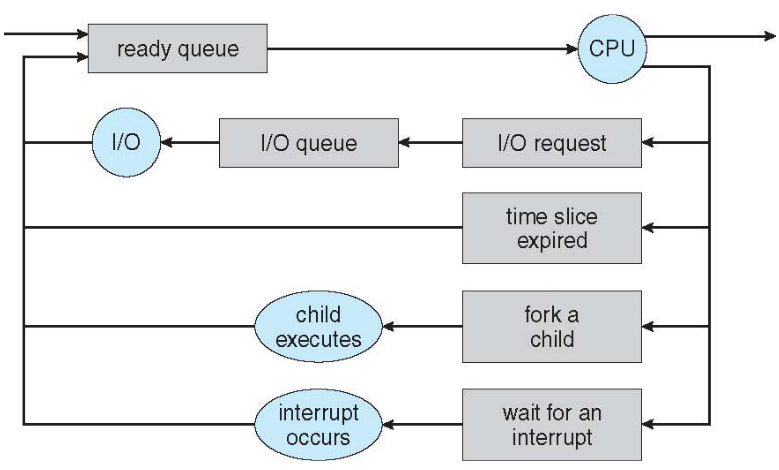
\includegraphics[width=8.2cm]{SO_PNGs/queueing-diagram_SO.png}
		\caption*{}
		\label{fig:queueing-diagram}
	\end{figure}
	

	\subsection*{InterProcess Communication (IPC)} 
	Un gruppo di system calls che implementa meccanismi di comunicazione e sincronizzazione dei processi. \\
	Due tecniche principali:
	\begin{itemize}
		\item uso di \textit{shared memory locations}, dove il kernel viene chiamato per creare l'area di memoria, dopodiché i processi possono comunicare tra loro senza dover chiamare il kernel ogni volta
		\item message passing (il kernel viene chiamato per la ``consegna'')
	\end{itemize}

	\subsection*{Producer} 
	Il buffer viene calcolato in maniera ``circolare''. Quando gli indicatori \textit{in} e \textit{out} sono sovrapposti, significa che il buffer è vuoto, contrariamente se il buffer è pieno, (?)hanno una determinata distanza(?) \\
	La sicnronizzazione consiste nel fermare il produttore se il buffer è pieno e fermare il consumatore e il buffer è vuoto. \\
	
	
	\subsection*{Threads}
	Implementati in risposta del bisogno di avere una maggiore capacità di calcolo. Permettono di eseguire multiple tasks per lo stesso fine, ergo esegue le stesse attività in maniera \textit{concorrente}. Prima dei threads questo si otteneva per mezzo dell'utilizzo di processi figli. Di conseguenza un thread viene utilizato per ricreare il concetto di processo figlio senza effettivamente doverne creare uno, permettendo di scrivere un unico programma con diversi punti di esecuzione che gestiscono il SO, agendo nella stessa area di memoria. \\ \\
	Sono implementati mediante:
	\begin{itemize}
		\item Librerie
		\item Supporto Hardware
		\item Architetture Multi-Core
	\end{itemize}
		
	\subsection*{Lezione 6 (Processor Scheduling)}
	
	I sistemi operativi permettono di mandare sul processore altri programmi mentre i programmi già presenti sono in stato di attesa. Questo permette che l'esecuzione di più processi avvenga nel modo più fluido ed efficiente possibile. \\ 
	
	\begin{figure}[!htbp]
		\centering
		\begin{subfigure}{.3\textwidth}
			\centering
			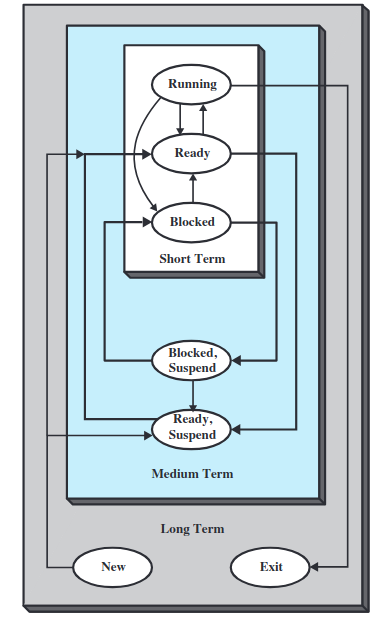
\includegraphics[width=4cm]{SO_PNGs/levels-of-scheduling_SO.png}
			\caption*{}
			\label{fig:levels-of-scheduling}
		\end{subfigure}%
		\begin{subfigure}{.7\textwidth}
			\centering
			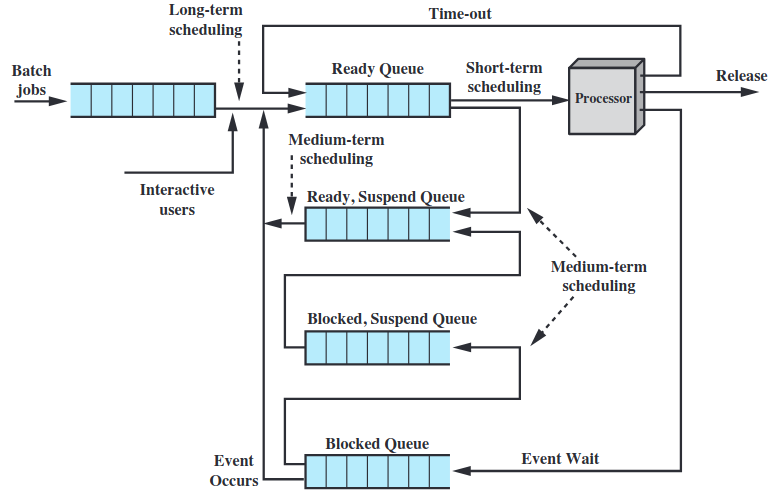
\includegraphics[width=12cm]{SO_PNGs/queueing-diagram-scheduling_SO.png}
			\caption*{}
			\label{fig:queueing-diagram-scheduling}
		\end{subfigure}%
		
	\end{figure}

	
	\subsection*{Short term Scheduling}
	
	\begin{itemize}
		\item La multiprogrammazione permette di massimizzare l'utilizzo della CPU
		\item \textbf{CPU-I/O Burst Cycle}: L'esecuzione di un processo consiste in un ciclo di esecuzione in CPU e di attesa di I/O
		\item Il CPU burst viene seguito da un \textit{I/O Burst} 
	\end{itemize}
	La distribuzione della CPU Burst è di principale interesse
	
	\begin{itemize}
		\item \textbf{CPU Bound}
		\item \textbf{I/O Bound}
	\end{itemize}

	Lo Short Time Scheduling si occupa delle operazioni di Ready e di Run. \\
	I processi di Run sono interrotti sono il caso di un'operazione di Exit, di Block o quando interviene il SO. Il movimento di un programma da Run a Ready viene appunto preso in carico dal SO.
	\\
	L'obiettivo è di allocare tempo al processore in modo da ottimizzare alcuni aspetti del comportamento del sistema. Ci sono due criteri per valutare lo Scheduling: 
	\begin{itemize}
		\item \textbf{User-Oriented Criteria}: in relazione al comportamento del sistema come percepito dall'utente o dal processo (es. tempo di risposta)
		\item \textbf{System-Oriented Criteria}: Focus su l'effettivo ed efficiente utilizzo del processore, generalmente di minore importanza sui sistemi a singolo utente.
	\end{itemize}
	
	Le prestazioni si possono misurare in maniera quantitativa o qualitativa.
	\begin{itemize}
		\item \textbf{Max CPU utilization}: Utilizzo della CPU
		\item \textbf{Max throughput}: Numero di processi che completano la loro esecuzione ogni unità di tempo
		\item \textbf{Min Turnaround Time}: Quantità di tempo per eseguire un certo processo
		\item \textbf{Min Waiting Time}: Quantità di tempo che un processo ha passato attendendo in ready queue
		\item \textbf{Min Response Time}: Quantità di tempo richiessto da quando una richiesta viene inviata fino a quanto la prima risposta viene prodotta
	\end{itemize}
		
	Vengono utilizzati degli \textbf{algoritmi} per poter misurare queste quantità:
	\begin{itemize}
		\item \textbf{First-Come First-Served (FCFS)}
		\begin{itemize}
			\item Detto anche First-In First-Out o Scrict Queuing Scheme, è la tecnica di scheduling più semplice (data l'implementazione facile e la sua velocità)
		\end{itemize}
:	\end{itemize}
	// ADD FCFS Example Slide (Esercizio) // \\ \\
	\begin{itemize}
		\item \textbf{Shortest Process Next (SPN)}
			\begin{itemize}
				\item Il processo con il tempo previsto più corto viene selezionato come successivo
			\end{itemize}
		\item \textbf{Shortest Remaining Time (SRT)}
			\begin{itemize}
				\item Il processo in run può essere svuotato dal nuovo processo che si sta unendo alla ready-queue se la sua CPU-Burst è più piccola della CPU-Burst del processo in run.
			\end{itemize}
	\end{itemize}
	// ADD SRT Slide // \\ \\
	Un \textit{priority number} (integer) viene associato con ogni processo, viene calcolato dal SO e impostato dall'utente. In Linux più un processo diventa anziano, più il suo valore di priorità viene incrementato (il commando ``nice'' in linux permette di impostare la priorità di un processo). Di conseguenza diventa conveniente implementare uno scheduling basato sulla priorità:
	\begin{itemize}
		\item \textbf{Priority Scheduling}
		\item \textbf{Round Robin (RR)}: Scheduling circolare, ogni processo ottiene una piccola unità di tempo di CPU (time quantum q), generalmente 10-100 millisecondi. Dopo che questa unità di tempo scade, il processo viene svuotato e viene messo alla fine della ready-queue. Il successivo processo in queue viene eseguito. \\
		Se ci sono $n$ processi nella ready-queue e \textit{quantum time} $q$, nessun processo di conseguenza dovrà aspettare più di $q(n-1)$ unità di tempo.
	\end{itemize}
	// ADD RR example Slide // \\ \\
	
	
	\subsection*{Multilevel Queue Scheduling}
	Il SO sceglie l'algoritmo di scheduling più appropriato in base a ciascuna queue.
	
	
	\subsection*{Multiple-Processor Scheduling}
	Il primo processore libero viene occupato
	
	
	\section*{Lab 3 Linux}
	
	Ogni processo in Linux è generato da un processo \textbf{padre}, ogni processo, di conseguenza avrà un certo PPID (parent process identifier). \\ Si può vedere ogni processo attivo nella macchina usando il comando ``ps -el'' \\
	Il SO ha bisogno di un syscall per creare un nuovo processo, si usa fork() per questo. fork() ha dei valori di ritorno:
	\begin{itemize}
		\item 0, al processo figlio
		\item PID del Figlio, al processo padre
		\item -1, nel caso in cui la syscall fork fallisca
	\end{itemize}
	Il fork() crea un'esatta copia del processo, ritornando un valore di 0 al figlio, il PID al processo padre.
	
	
	\section*{Lezione 7}
	
	// FCFS Algorithm image exercise // \\ \\
	
	// SPN Image ex. // \\\\
	Shortest Process Next (SPN): significa che la durata di ogni processo viene \textit{stimata}. L'ordine dei processi varia in base alla loro durata (in quanto il focus dell'algoritmo è di ridurre l'attesa dei processi più corti).
	\\ \\ \\
	// SRT Ex.  // \\ \\
	Shortest Remaining Time (SRT): è un algoritmo pre-emptive. Quando c'é una coda di processi lo scheduler guarda se il processo nella coda richiede meno tempo di quello in running e se ha un valore di priorità maggiore(nel caso in cui l'algoritmo lo prendesse in considerazione, nel caso dell'esempio, la priorità viene ignorata). \\ \\ 
	// RR ex // \\ \\
	Round Robin (RR) [q = 4]: ogni processo viene eseguito ogni $q$ unità di tempo (q = 4 in questo caso) e viene poi rimesso in coda. 
	\\ \\ \\ 
	Real-Time Operating Systems\\ 
	Devono essere
	\begin{itemize}
		\item Deterministici
		\item Responsivi 
		\item Utilizzabili dall'utente
		\item Affidabili
		\item Essere a prova di errori
	\end{itemize}
	Hanno algoritmi di scheduling come:
	\begin{itemize}
		\item Round-Robin (...)
		\item A (...)
		\item Priority-Driven Pre...
		\item (...)
	\end{itemize}

	
	\section*{Lezione 8}
	
	Classi di RTOS
	\begin{itemize}
		\item Static table-driven approaches
		\item Static priority-driven preemptive approaches
		\item Dynamic planning-based approaches
		\item Dynamicc best effort approaches (Più frequenti negli RTOS commerciali)
	\end{itemize}


	\subsection*{Informazioni usate per lo Scheduling}
	\begin{itemize}
		\item Ready time
		\item Starting Deadline
		\item Completion Deadline
		\item (...)
		\item Resource requirements
		\item Priority
		\item Subtask Scheduler
	\end{itemize}
	
	
	\subsection*{Unbounded Priority Inversion (Inversione di Priorità)}
	
	(...)
	\\
	
	
	\subsection*{Concorrenza}
	I processi possono overlappare ed intrecciarsi, e la loro \text{velocità relativa di esecuzione} non può essere predetta nei sistemi uniprocessore.
	\\
	Si ha un rapporto Producer/Consumer, dove le risorse vengono prodotte per poi essere consumate da qualcun'altro.
	
	\begin{lstlisting}[language=C]
	// PRODUCER
	while (true) {
		\* produce an item in next_product */
		while (count == DIM_BUFFER)
			/* do nothing */
		buffer[in] = next_product;
		in = (in + 1) % DIM_BUFFER;
		count++;
	}

	// CONSUMER
	while (true) {
		while (count == 0)
			/* do nothing */;
		next_consumed = buffer[out];
		out = (out + 1) % DIM_BUFFER;
		count--;
		/* consume an item in next_consumed */
	}
	\end{lstlisting}

	Se i processi di Producer/Consumer si overlappano, risulterà un errore.
	
	
	\subsection*{Critical Section}
	
	Ogni protocollo che indirizza la sezione critica deve soddisfare il progresso, la mutua esclusione e i limiti d'attesa. \\
	Si può arginare il problema dei process che si sovrascrivono attraverso degli algoritmi appositi. \\
	Di seguito, è descritto \textbf{l'Algoritmo di Peterson} per un Processo $P_i$:
		
	\begin{lstlisting}[language=C]
	do {
		flag[i] = true;
		turn = j;
		while (flag[j] && turn == j);
			critical section
		flag[i] = false;
			/* remainder section */
	} while (true);
	\end{lstlisting}

	Due processi $P_i$ e $P_j$, dove $i = 1 - j$ \\
	Variabili condivise: \\
	\textbf{int turn;}  \\
	\textbf{boolean flag[2];}
	
	
	
	\section*{Lezione 9}
	
	\subsection*{Semafori}
	Ogni semaforo funziona come waiting queue per più processi
	\begin{lstlisting}[language=C]
	wait(semaphore *S) {
	  S -> value++;
	  if ( S -> value <= 0 ) {
	  	// Code...
  	  }
  	}
	\end{lstlisting}
	
	-BACI - Ben Ari Concurrent Interpreter \\ \\
	L'implementazione dei semafori ha una serie di problemi standard:
	\begin{itemize}
		\item \textbf{Deadlock}: (o stallo) condizione dove nessun processo può avanzare.
		\begin{lstlisting}
	P_0			P_1
	wait(S);		wait(Q);
	wait(Q);		wait(S);
	...				...
	signal(S);		signal(Q);
	signal(Q);		signal(S);
		\end{lstlisting}
		
		\item \textbf{Sincronizzazione}: 
			\begin{itemize}
				\item \textit{Bounded buffer Produttore/Consumatore}: sia il produttore che il consumatore scrivono nello stesso Buffer, creando problemi di memoria\\
				Una soluzione può essere riservare il buffer al produttore finché non è pieno. Se non ci sono celle disponibili, il consumatore deve aspettare.
				\item \textit{Readers/Writers problem}: un'area di memoria viene \textit{condivisa} tra più processi, alcuni leggono soltanto (readers), altri invece scrivono (writers). \\
				Le condizioni che vanno soddisfatte sono dunque:
				\begin{itemize}
					\item Tutti i readers possono leggere simultaneamente un file
					\item Solo un writer alla volta può scrivere nel file
					\item Se tutti i writer scrivono nel file, nessun reader può leggerlo
				\end{itemize}
				\item \textit{Dining Philosophers problem}: Cinque filosofi a cena, spendono il loro tempo alternando l'atto di mangiare e di pensare. Condividono tra loro una ciotola di spaghetti e delle forchette. Ogni filosofo alla fine si ritrova con una forchetta a sinistra ed una sulla destra. \\
				Il fulcro del problema è che \textit{non esiste} una soluzione ottimale. \\\\
				Per evitare un deadlock, si possono attuare delle restrizioni:
				\begin{itemize}
					\item Solo uno dei cinque filosofi può richiedere le forchette
					\item Le forchette devono essere prese in paio e non una alla volta
					\item Ogni filosofo che occupa una posizione \textit{dispari} prende prima la forchetta a sinistra e dopo quella a destra. Ogni filosofo che occupa un posto \textit{pari} invece prende prima la destra e poi la sinistra
				\end{itemize}
			\end{itemize}
	\end{itemize}


	\section*{Lezione 10}

	\subsection*{Monitor}
	
	E' un costrutto di sincronizzazione che impedisce ai threads di accedere simultaneamente ad uno stesso oggetto condiviso. \\
	(...) \\
	\\ append(), producer \\
	take(), consumer (...) \\ \\ \\
	
	// Structure of a monitor with condition variables image // \\ \\
	
	Mutua esclusione, i processi in coda sono bloccati.
	
	\subsection*{Concurrency: Deadlock and Starvation}
	
	Per capire il Deadlock, si può considerare ogni processo come un'entità che può richiedere o mantenere delle risorse. Dato un set di processi, il set è in deadlock se il meccanismo smette di muoversi.
	\\ \\
	Le condizioni per un deadlock sono
	\begin{itemize}
		\item Mutua Esclusione
		\item Hold-and-Wait
		\item No Pre-emption
		\item Circular Wait
	\end{itemize}
	Sono tutte condizioni sufficienti affinché si verifichi un deadlock. \\
	Non esiste una soluzione generale a questo problema, tuttavia esistono delle strategie che si possono applicare a tutti i tipi di deadlock (stallo). Ci sono tre approcci comuni:
	\begin{itemize}
		\item Prevenzione dello stallo: disabilita una delle tree condizioni necessarie per lo stallo
		\item Evitare lo stallo: previene l'accesso ad una delle risorse
		\item Rilevazione dello stallo: (...)
	\end{itemize}
	Altri due approcci per la prevenzione di stalli:
	\begin{itemize}
		\item Resource Allocation Denial: conosciuto anche come \textbf{Banker's Algorithm}, cerca di predirre lo stato del processo per portarlo ad uno stato di sicurezza
		\item Deadlock Detention: algoritmi che rilevano lo stallo
	\end{itemize}
	Il recupero dallo stallo si può ottenere fermando tutti i processi in stallo, in base alla priorità, l'importanza, etc... del processo. Recovery (...). 
	
	
	\section*{Lezione 11. Pipes}
	
	\section*{Lezione 12}
	
	I programmi devono essere portati dal disco nella memoria e messi in un processo per poter essere eseguiti. La gestione della memoria ci serve per azione di rilocazione, protezione ( fare in modo che i programmi non interferiscano l'un l'altro), apetti di condivisione dei dati. Un processo già in esecuzione non ha bisogno di essere rilocato, a meno che più programmi vengano avviati, in tal senso allora la memoria necessita di rilocare i processi. Ci sono diverse tecniche attuate per la rilocazione. \\ 
	La protezione dei processi si attua avendo nel processore una sorta di 'tabella' nel quale viene memorizzato l'inizio e la fine ( in termini di indirizzi di memoria ) dei vari processi in run. \\
	Il concetto di condivisione invece è complementare a quello di protezione, ovvero può capitare che alcuni programmi abbiano bisogno di una certa risorsa ( es. librerie DLL), di conseguenza allora una volta messa in memoria la risorsa verrà condivisa a tutti i processi che ne hanno bisogno. \\
	I programmi vengono scritti in moduli, ed anche la memoria principale tende ad avere la stessa organizzazione logica, ovvero è divisa in \textbf{segmenti}, ciscuno corrispondente ad i moduli dei programmi. \\
	Generalmente il programmatore non può gestire la memoria, poiché non sa quanto spazio dovrà occupare un determinato programma, inoltre la memoria necessaria per un programma ed i suoi dati potrebbe non essere sufficiente.(?) L'overlaying è una tecnica che permette di segmentare un programma e riassemblarlo in base alle necessità (?) \\
	Il calcolo degli indirizzi può avvenire in 3 stages(?): 
	\begin{itemize}
		\item Compile time: se l'area di memoria si conosce a priori, il codice assoluto può essere generato
		\item (...)
		\item (...)
	\end{itemize}
	Il SO gestisce degli indirizzo logici che sono confinati da un indirizzo fisico separato, gli indirizzi logici sono generati dalla CPU (indirizzi virtuali), gli indirizzi fisici sono invece visti dall'unità di memoria. \\
	Gli indirizzi logici e fisici sono identici in compile-time e load-time (?) \\
	Gli indirizzi logici(virtuali) e fisici differiscono in execution-time address binding scheme (??) \\\\
	
	
	\subsection*{Swapping}
	
	Tecnica ( usata molto negli anni '90, implementata tutt'oggi in maniera simile negli smartphones ), e' simile allo stato di bloccato, ed un programma viene messo in 'stasi' e poi rimesso in esecuzione quando riportato in primo piano ( similmente allo swap delle applicazioni in esecuzione degli smartphone ). Non tiene in programma l'.exe, ma tiene in memoria lo stato del processo all'ultimo istante. 
	
	\subsection*{Memory Partitioning}
	
	Allocazione Contigua: ovvero all'avvio il SO viene caricato sempre nella stessa locazione nella memoria principale, dopodiché tutti i processi successivi vengono caricati in successione, il problema è che se termina un processo, potrebbe lasciare buchi in memoria. Questa implementazione è perfetta dal punto di vista dell'esecuzione dei programmi. Il problema è appunto, la differenza di dimensioni dei programmi, che lasciano buchi di memoria alla fine dell'esecuzione. Quindi il buco di memoria lasciato da un programma potrebbe non essere sufficientemente grande per lasciare spazio ad un'altro programma.  \\
	Qui nasce il problema della \textbf{Dynamic Storage-Allocation}. Come soddisfare una richiesta di dimensione $n$ da una lista di buchi liberi?
	\begin{itemize}
		\item First-fit: Alloca il primo buco che è grande abbastanza
		\item Best-fit: Alloca il buco più piccolo, che però è grande abbastanza ( richiede però di stilare una lista in base alla grandezza dei buchi )
		\item Worst-fit: Alloca il buco più grande possibile (deve comunque scorrere l'intera lista)
	\end{itemize}
	
	\subsection*{Segmentation}
	
	Il concetto di segmentazione rende il SO più complicato, però al contempo più efficiente. La segmentazione è la divisione di ogni programma in segmenti, dove un segmento è un'unità logica come:
	\begin{itemize}
		\item programma principale
		\item procedura
		\item funzione
		\item metodo
		\item oggetti
		\item variabili locali, variabili globali
		\item blocchi comuni
		\item stack
		\item tavola dei simboli (symbol table)
		\item arrays
	\end{itemize}
	Perciò il SO non vede il programma come un monolite, ma vede le varie segmentazioni. In memoria perciò i segmenti non saranno allocati necessariamente in maniera contigua, ma saranno a loro volta allocati in parti diverse. Tuttavia il SO dovrà accessoriarsi di una tabella dei segmenti per ogni processo, dove ogni tavola ha una \textbf{base} ed un \textbf{limite}. \\\\
	// Example of Logical-to-Physical Address Translation // \\ \\
	
	
	\subsection*{Paging}
	
	Un altro meccanismo accoppiato a quello della segmentazione è quello della paginazione. La tecnica della paginazione permette di gestire la memoria principale logicamente suddivisa in pagine, il problema è che la dimensione delle pagine è statica, e la suddivisione in pagine potrebbe tagliare a metà anche delle istruzioni. \\
	Partizioniamo la memoria in chunks di uguale dimensione (di grandezza relativamente piccola), e dividiamo anche il processo in chunks di stessa dimensione.
	
	
	
	\section*{Lezione 13}
	(...)
	
	
	
	\section*{Lezione 14}
	(...)
	
	
	
	\section*{Lezione 15}
	
	
	
	
\end{document}

